\documentclass[11pt,a4paper]{article}
\usepackage{times}
\usepackage{latexsym}
\usepackage{url}
\usepackage{color}
\usepackage{graphicx}
\usepackage{cjhebrew}
\usepackage[T2A,OT2,OT1]{fontenc}
\usepackage{ucs}
\usepackage{CJKutf8}
\usepackage{footnote}
\usepackage{caption}

% \usepackage{float}
\usepackage{subfigure}

% \usepackage{subfig}
\usepackage{floatrow}
% \floatsetup[figure]{style=plain}

\usepackage[hebrew,english]{babel}
\newcommand{\heb}[1]{%
  \foreignlanguage{hebrew}{#1} }

\newcommand\cyr{%
\renewcommand\rmdefault{wncyr}%
\renewcommand\sfdefault{wncyss}%
\renewcommand\encodingdefault{OT2}%
\normalfont
\selectfont}
\DeclareTextFontCommand{\textcyr}{\cyr}
\usepackage{acl2014}

\newcommand{\ddcomment}[1]{\textcolor{red}{[$^{\textsc{D}}_{\textsc{D}}$ #1]}}
\newcommand{\spcomment}[1]{\textcolor{blue}{[$^{\textsc{S}}_{\textsc{P}}$ #1]}}
\newcommand{\jmcomment}[1]{\textcolor{magenta}{[$^{\textsc{J}}_{\textsc{M}}$ #1]}}
\newcommand{\eat}[1]{\ignorespaces}

\newcommand{\query}[1]{\texttt{#1}}

\setlength\titlebox{6.5cm}    % Expanding the titlebox

\title{Enhanced Search with Wildcards and Morphological Inflections\\in the Google Books Ngram Viewer}

\eat{\author{Jason Mann, David Zhang, Lucille Yang, Slav Petrov and Dipanjan Das\\
	Google Inc. \\
	{\tt jcm2207@columbia.edu, dzhang21@gmail.com, ly77@cornell.edu}\\
	{\tt \{slav,dipanjand\}@google.com}}
}

\date{}

\begin{document}
\maketitle

\begin{abstract}

We present a new version of the Google Books Ngram Viewer, which plots
the frequency of words and phrases over the last five
centuries; its data encompasses 6\% of the world's published books.
The new Viewer adds three features for more powerful search: wildcards,
morphological inflections, and capitalization. These additions allow
the discovery of patterns that were previously difficult to find in the Google Books Ngram data,
and further facilitate the study of linguistic trends in printed text.

\end{abstract}

\section{Introduction}

The Google Books Ngram project facilitates the analysis of cultural, social and linguistic trends through five centuries of written text in eight languages. The Ngram Corpus \cite{culturomics,lin2012syntactic} consists of words and phrases (i.e., ngrams) and their usage frequency over time; it is freely available for download. The interactive Ngram Viewer\footnote{See \url{http://books.google.com/ngrams}.} allows users to retrieve and plot the frequency of multiple ngrams on a simple webpage. The Viewer is widely popular and can be used to efficiently explore and visualize patterns in the underlying ngram data. For example, the ngram data has been used to detect emotion trends in 20th century books \cite{acerbi.etal.2013}, to analyze text focusing on market capitalism throughout the past century \cite{Schulz2013}, detect social and cultural impact of historical personalities \cite{skiena.ward.2013}, or to analyze the correlation of economic crises with a literary `misery index' reflected in printed text during crises periods \cite{bentley.et.al.2014}.



\begin{figure}
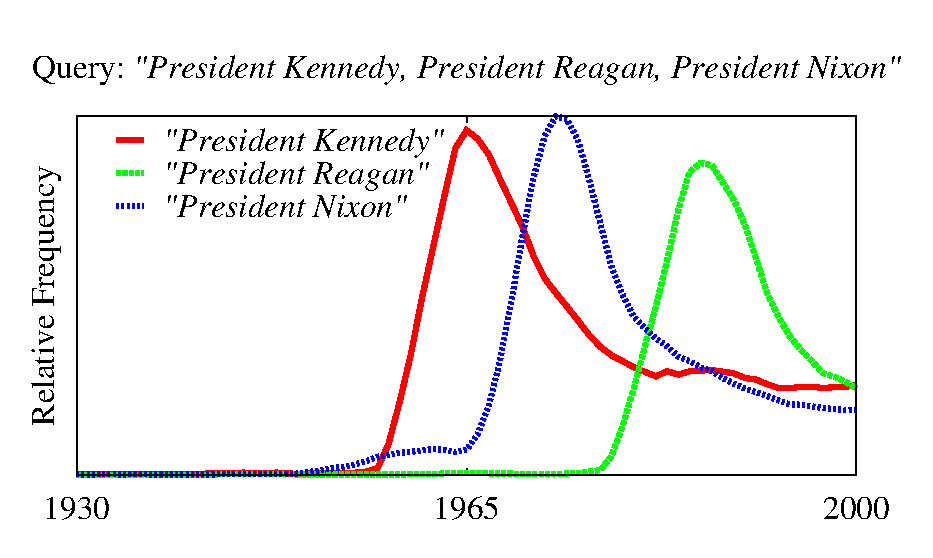
\includegraphics[width=\columnwidth]{graphs/kenreanixon}
\caption{\label{fig:manual president} Manual query of president's names}
\end{figure}

A major limitation of the Ngram Viewer, however, is that all the reasoning have to be carried out by the user, and that the Viewer cannot automatically discover interesting trends. For example, to compare the popularity of different presidents, one might search for `\query{President Kennedy, President Nixon, President Reagan}', and so forth. In order to determine the most popular president, one would need to search for all presidents, which is cumbersome and should ideally be automated.

% \begin{savenotes}
% \begin{figure*}
% 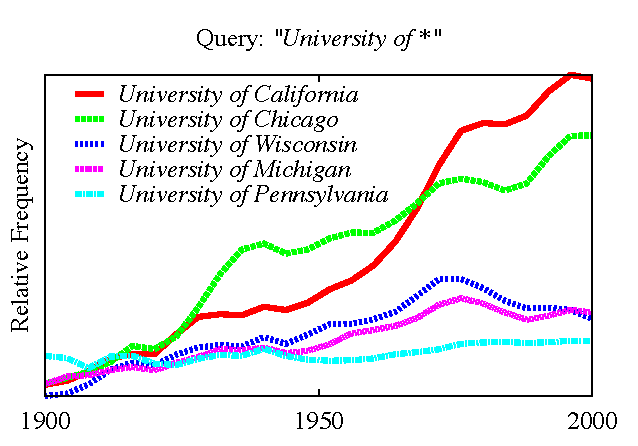
\includegraphics[width=0.49\textwidth]{graphs/university}\hspace{2\unitlength}%
% 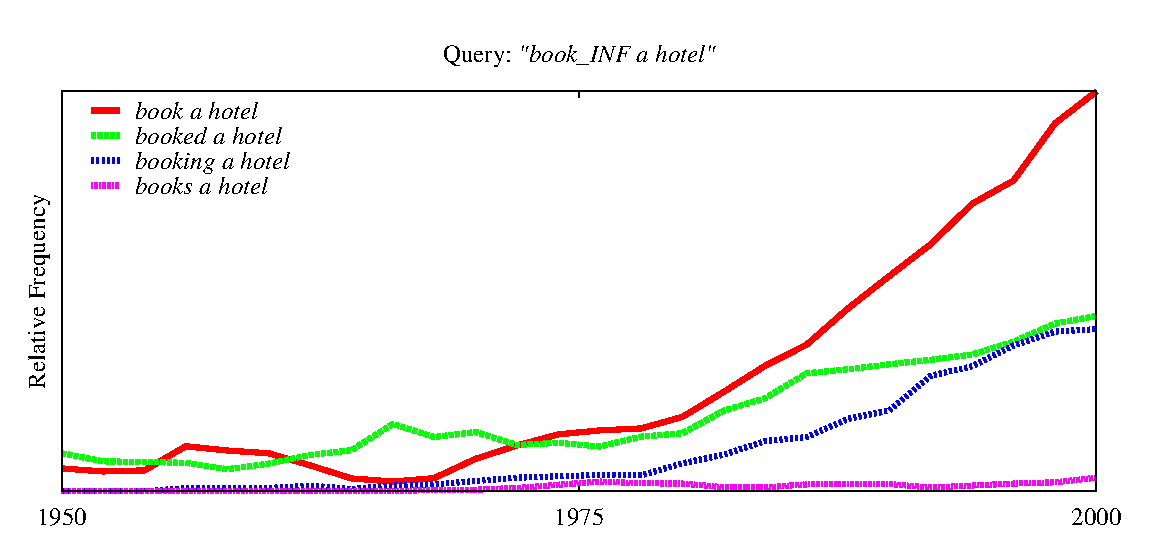
\includegraphics[width=0.49\textwidth]{graphs/book}\vspace{2\unitlength}\par
% 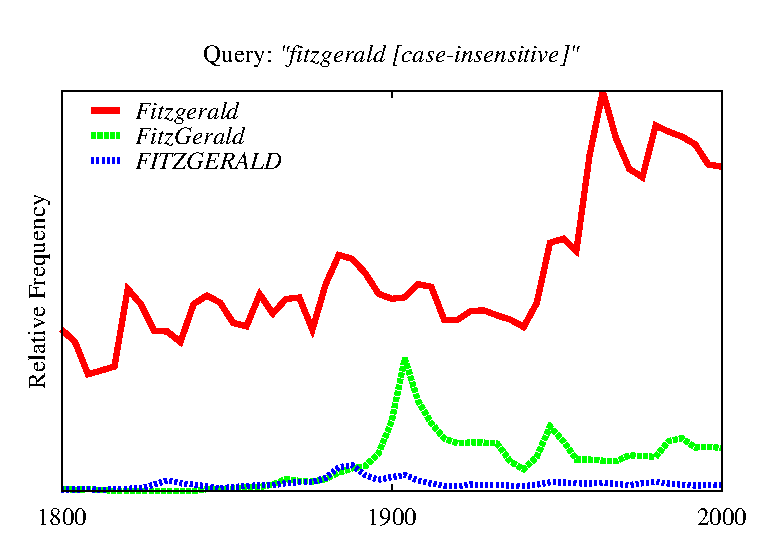
\includegraphics[width=0.49\textwidth]{graphs/fitzgerald}\hspace{2\unitlength}%
% \parbox[b][]{.49\textwidth}%
% {\RawCaption{
% \caption{In the new enhanced search a single query is automatically expanded to retrieve multiple related ngrams.\footnotemark{}}\label{fig:examples}}}
% \end{figure*}
% \footnotetext{These figures show fewer results than returned by the Ngram Viewer due to space considerations.}

\begin{figure*}[t]
\centering
\addtolength{\subfigcapskip}{-0.2cm}
\hspace*{-0.5cm}
\subfigure[Wildcard example.]{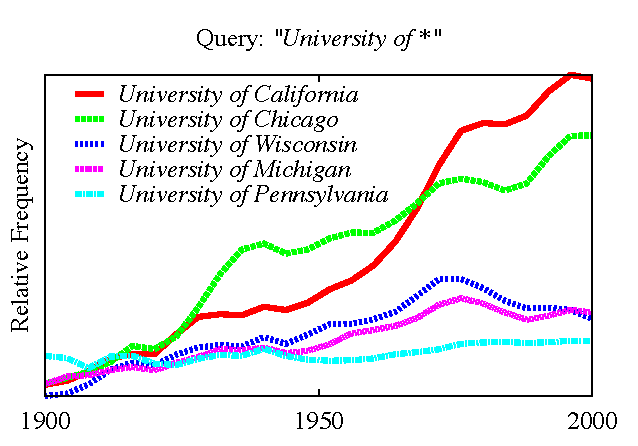
\includegraphics[width=0.49\textwidth]{graphs/university}}
\hspace*{0.1cm}
\subfigure[Inflection example.]{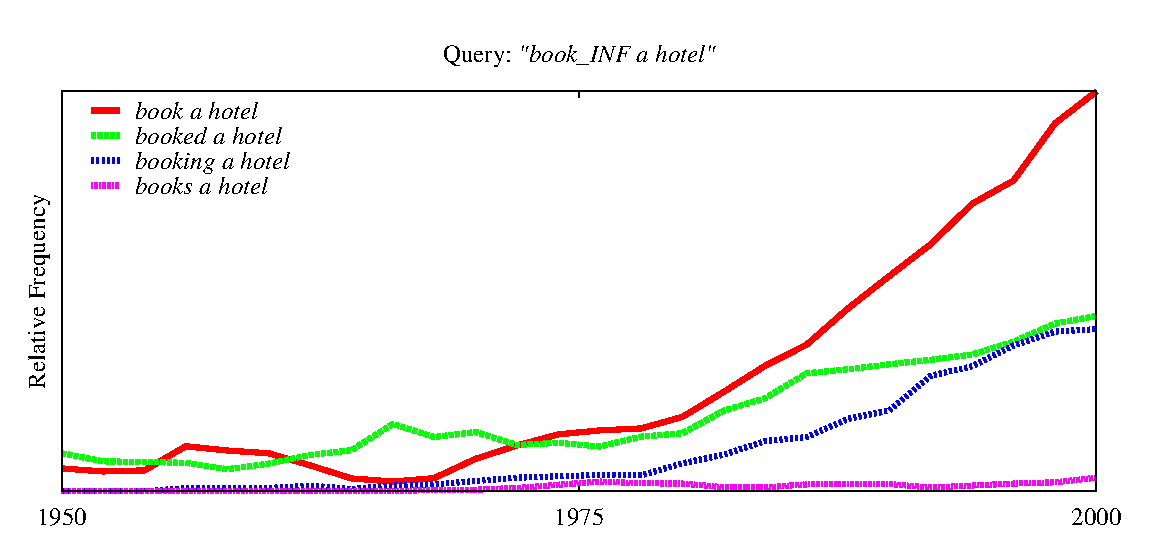
\includegraphics[width=0.49\textwidth]{graphs/book}}

\hspace*{-0.5cm}\vspace*{-0.3cm}
\subfigure[Capitalization example.]{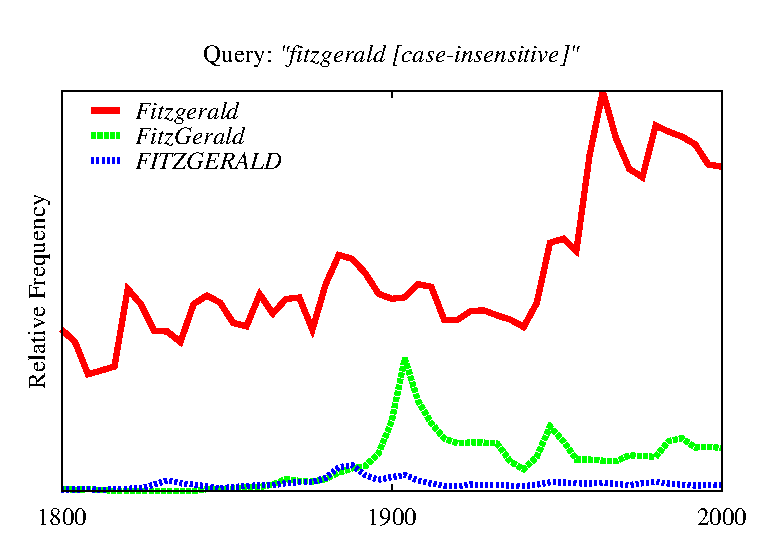
\includegraphics[width=0.49\textwidth]{graphs/fitzgerald}}
\hspace*{0.1cm}
\parbox[b][]{.49\textwidth}%
{\RawCaption{\caption{\label{fig:examples}
In the new enhanced search features of the Ngram Viewer presented in this paper, a single query is automatically expanded to retrieve multiple related ngrams.\footnotemark{} The
wildcard operator `\query{*}' is shown in (a), (b) shows the usage of the `\query{\_INF}' marker that results in morphological
inflections, while the case-insensitive
search functionality is shown in (c).}}}
\end{figure*}
\footnotetext{We show fewer results in this figure than the ones returned by the Ngram Viewer due to space considerations.}

In this paper, we therefore present an updated version of the Viewer that enhances its search functionality. Traditional searches retrieve and plot the frequency of individual, user-specified ngrams. Instead, the three new features that we introduce automatically expand a given query and retrieve a collection of ngrams, to facilitate the discovery of patterns in the underlying data. First, users can replace one query term with a placeholder symbol `\query{*}' (wildcard, henceforth), which will return the ten most frequent expansions of the wildcard in the corpus for the specified year range. 
%Figure~\ref{fig:examples}(a) shows the automatically discovered increase in references to the University of California. 
Second, by adding a specific marker to any word in a query (`\query{\_INF}'), ngrams with all morphological inflections of that word will be retrieved. 
%Figure~\ref{fig:examples}(b) shows the four inflected forms of the word book in the ngram `book a hotel'.
Finally, the new Viewer supports capitalization searches, which return all capitalization variants of the query ngram. Figure~\ref{fig:examples} provides examples for these three new types of queries.
%Figure~\ref{fig:examples}(c) shows the decline in the camel-case spelling of the surname Fitzgerald.
% Slav: we could discuss the examples in Fig. 1 here.

While it is fairly obvious how the above search features can be implemented via brute-force computation, supporting an interactive application with low latency necessitates some non-trivial engineering. In particular, the wildcard search feature poses some challenges because the most frequent expansions depend on the selected year range (consider the frequency with which presidents are mentioned during different decades, for example). To this end, we provide details on our system architecture in \S\ref{sec:overview}  and discuss how the new search features are implemented in \S\ref{sec:features}.
% We could add a sentence summarizing how we deal with wildcards here.

In addition, this demonstration presents an overhaul of the Viewer's user interface (\S\ref{sec:interface}), with interactive features that allow for easier management of the increase in data points returned. For example, to normalize for morphological inflections or casing, the frequencies of multiple ngrams can be aggregated via a (right) mouse-click. Additionally, lines can be highlighted or faded (via hovering or mouse-clicks) to focus on particular ngrams and make trends more apparent.

Detailed analysis and interpretation of trends uncovered with the new search interface is beyond the scope of this paper. We include some interesting use cases in \S\ref{sec:usecases}; many of the presented queries were difficult (or even impossible) to execute in the previous versions of the Ngram Viewer. We hope the presented functionalitied of the Viewer will help uncover trends and patterns not readily apparent in the Ngram Corpus.\ddcomment{The last line could be in the conclusion section.}

\section{System Overview}
\label{sec:overview}

We start by presenting an overview of the system architecture. We briefly review the underlying corpus and architecture of previous versions of the Viewer \cite{culturomics,lin2012syntactic} and then focus on the extensions added in this version. It should be emphasized that this demonstration updates only the Viewer, and provides tools for easier analysis of the underlying data. The ngram data itself is not updated and is identical to that of \newcite{lin2012syntactic}.


\subsection{Ngram Corpus}
	The Google Books Ngram Corpus\footnote{Downloadable from \texttt{https://books.google.com/} \texttt{ngrams/datasets}.} provides ngram counts for eight different languages over more than 500 years; additionally, the English corpus is split further into British vs. American English and Fiction to aid domain restriction. This corpus is a subset of all the books digitized at Google, and represents more than 6\% of all publicized texts \cite{lin2012syntactic}. Two editions of corpus are available: the first edition dates from 2009 and is described in \newcite{culturomics}; the second edition is from 2012 and is described in \newcite{lin2012syntactic}. Our new features are available for both editions.

\newcite{culturomics} extract ngrams for each page in isolation. More specifically, they use whitespace tokenization and extract all ngrams up to length five. These ngrams include ngrams that potentially span sentence boundaries, but do not include ngrams that span across page breaks (even when they are part of the same sentence).
\newcite{lin2012syntactic} on the other hand perform tokenization, text normalization and segmentation into sentences based on manually devised rules\footnote{Excluding Chinese, where a statistical segmentation system is used}. They then add synthetic \textsf{\textsc{\_start\_}} and \textsf{\textsc{\_end\_}} tokens to the beginning and end of the sentences to enable the distinction of sentence medial ngrams from those near sentence boundaries \cite{lin2012syntactic}. They also make sure to include sentences that span across page boundaries. Due to these differences, as well as the availability of additional book data, improvements to the optical character recognition algorithms and metadata extraction for dating the books, the ngrams counts from the two editions are not the same.

The edition from \newcite{lin2012syntactic} additionally includes syntactic ngrams. The corpus is tagged using the universal part-of-speech (POS) tag set of \newcite{petrov2012universal}: `\query{\_}': \query{NOUN} (nouns), \query{VERB} (verbs), \query{ADJ} (adjectives), \query{ADV} (adverbs), \query{PRON} (pronouns), \query{DET} (determiners and articles), \query{ADP} (prepositions and postpositions), \query{CONJ} (conjunctions). Words can be disambiguated by their POS tag by simply appending the tag to the word with an underscore (e.g. \texttt{book\_NOUN}) and can also be replaced by POS tags in the ngrams, see \newcite{lin2012syntactic} for details. The corpus is additionally parsed with a dependency parser and head-modifier syntactic relations between words in the same sentence are extracted. Dependency relations are represented as `\query{=>}' in the corpus. Our new enhanced search features for automatic expansions can also be applied to these syntactic ngrams. In fact, some of the most interesting queries use expansions to automatically uncover related ngrams, while using syntax to focus on particular patterns.

Finally, the Viewer supports the composition of ngram frequencies via arithmetic operators. Addition (\query{+}), subtraction (\query{-}) and division (\query{/}) of ngrams are carried out on a per year basis, while multiplication (\query{*}) is performed by a scalar that is applied to all counts in the time series. Where ambiguous the wildcard operator takes precedence over the multiplcation operator. Parentheses can be used for disambiguation and to force a particular interpretation.

\subsection{Architecture}
The Viewer provides a lightweight interface to the underlying ngram corpora. In its basic form, user requests are directed through the server to a simple lookup table containing the raw ngrams and their frequencies. This data flow is displayed in the top part of Figure \ref{fig:architecture} and is maintained for queries that do not involve the new expansion features introduced in this work.

The expansion queries could in principle be implemented by scanning the raw ngrams on the fly and returning the matching subset: to answer the query `\query{President *}', one would need to obtain all bigrams starting with the word \query{President} and extract the most frequent ten. Given the large quantity of ngrams, however, such an approach turns out to be computationally very expensive and too slow for an interactive application. We therefore pre-compute intermediate results that can be used to more efficiently retrieve the results for expansion queries. The intermediate results are stored in additional lookup tables (shown at the bottom in Figure \ref{fig:architecture}). When the user executes an expansion seqrch, the query is first routed to the appropriate intermedite results table which stores all possible expansions (including expansions that might not appear in the corpus).  These expanded ngrams are then retrieved from the raw ngram table, sorted by frequency and returned to he user.
%For example, the intermediate results table for the morphological variants search contains inflected forms for all unigrams. These inflected forms are substituted for the selected query term and the resulting ngram is looked up in the raw ngram table.
We describe the intermediate results tables and how they are generated in the next section.

It should be noted that we only support one expansion per query ngram. This is needed in order to avoid the combinatorial explosion that would result from mixing multiple expansions in the same ngram.

\begin{figure}
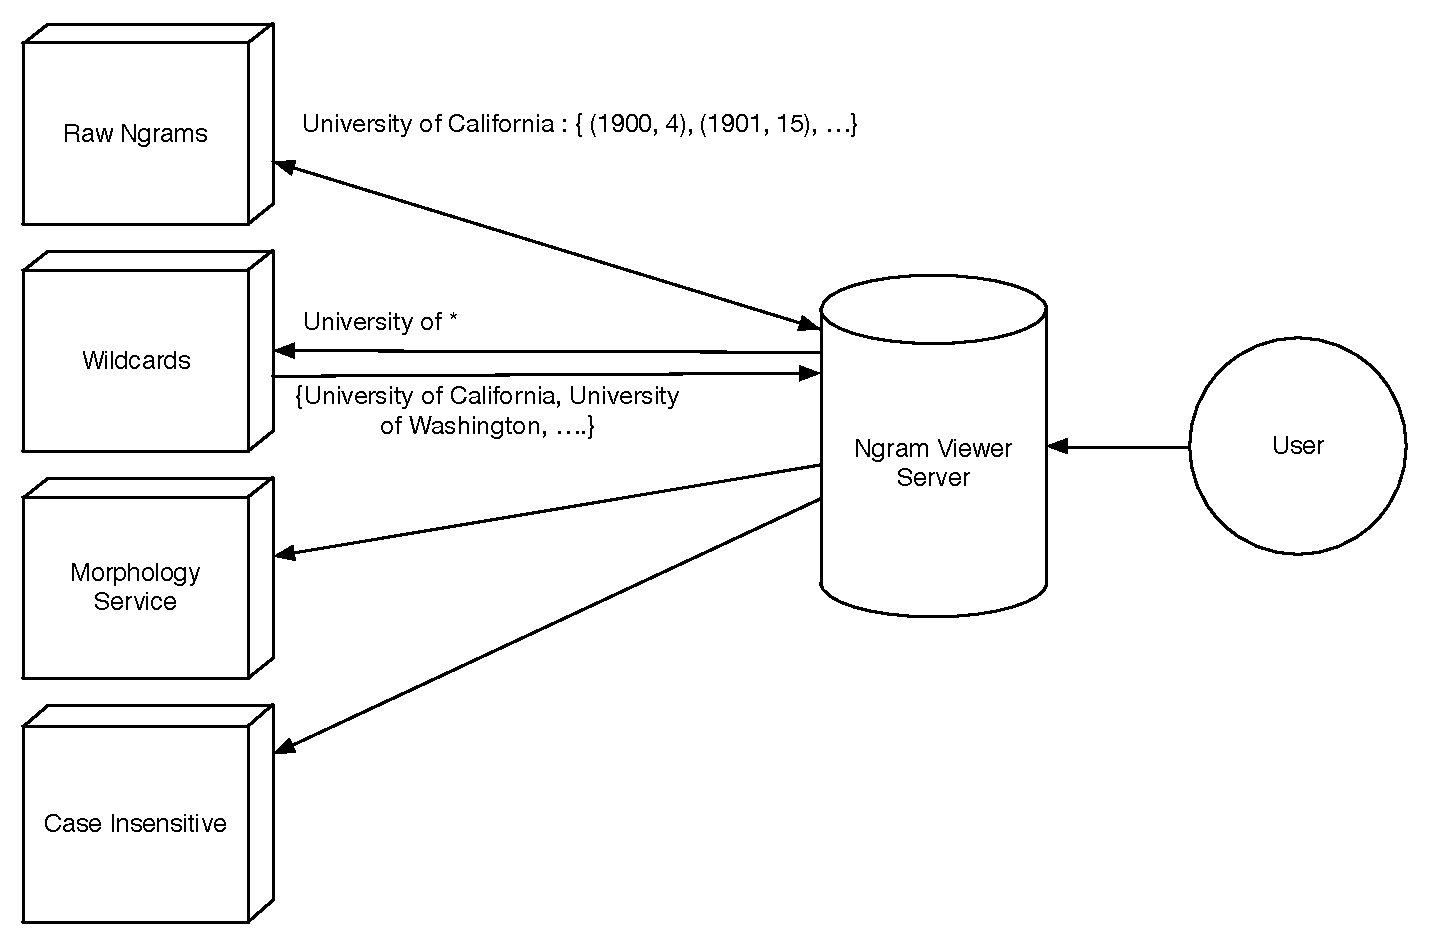
\includegraphics[width=\columnwidth,keepaspectratio=true]{system_architecture}
\caption{\label{fig:architecture}Diagram of new system architecture.}
\end{figure}


\section{New Features}
\label{sec:features}
Here, we describe the novel aspects of the Ngram Viewer introduced in this demonstration paper.
\begin{table*}
\small
\centering
\begin{tabular}{|c|c|}
\hline
\textbf{Query}	& \textbf{Possible Replacements}	\\ \hline \hline
\query{a * man}				& \query{a young man, a good man, a kind man, a wild man	}	\\ \hline
\query{booked=>*\_NOUN}	& 
\begin{tabular}[c]{@{}c@{}} \query{ booked=>flight\_NOUN, booked=>passage\_NOUN, }\\\query{booked=>room\_NOUN, booked=>eat\_NOUN}  \end{tabular} \\ \hline
\query{John said\_INF		}	& \query{John says, John said, John say, John saying} \\ \hline
\query{book\_INF\_NOUN		}	& \query{book, books     } \\ \hline
\begin{tabular}[c]{@{}c@{}} \query{the cook} (case insensitive)\end{tabular} & \query{THE COOK, the cook, The Cook, the Cook, The cook  } 	  \\ \hline
\end{tabular}
\caption{\label{tab:wildcard}
Examples of precompiled wildcard, inflection, and capitalization queries.}
\end{table*}


\subsection{Wildcards}
\label{sec:wildcards}
	We support the use of wildcards by utilizing an additional database that stores the most frequent expansions of queries to the ngram corpus. This wildcard database is created as a pre-compilation step when creating the Ngram Corpus from the Google Books data. When a new ngram is created, one word or tag at a time is replaced with the wildcard symbol, `*', creating a wildcard query. The query becomes a key in a string indexed lookup table, and the original ngram is added to a list of ngrams which are its values. As mentioned above, due to space considerations we were not able to store all possible expansions for every wildcard ngram we precomputed. Also, we could not precompute a perfect set of the top 10 ngrams for every possible year range, while this would require intermediate storage space on the order discussed above, as well as the computation time to calculate the top 10 for $\frac{n(n+1)}{2}$ time periods for each wildcard. Instead we estimate the top 10 during the creation of wildcard ngrams, by limiting the number of expansions to the top ten for every year. We gather these top 10 lists into a union and map the raw ngrams to the wildcard ngram string in our table. 
	
	During this process, we filter punctuation from consideration as a valid expansion because in practice punctuation returns uninteresting results. On this note, it may be useful to specify a specific POS tag (i.e. `*\textsf{\textsc{\_noun}}') to provide more specific results. At runtime, union of expansion ngrams is processed for the specific year range requested and the top ten results are returned. For examples of expansions see Table \ref{tab:wildcard}. 


\subsection{Morphological Inflections}
Inflections of words in search queries are handled using a Google Search interface that can provide morphological variations of words for different syntactic categories \cite{durrett2013supervised}. As this type of request utilizes an internal API, the results from a specific request are subject to change. Unlike wildcard substitutions, there is no need for pre-computation; given a query with the keyword \textsf{\textsc{\_inf}} attached to a word (e.g., `John said\textsf{\textsc{\_inf}}'), we get the counts of all the ngrams that start with `John' and have the morphological inflections of the root form `say' as its second word in the Ngram Corpus. We have noticed that there can be more than 10 results returned per query, especially for morphologically rich languages like Russian, unlike the wildcard search feature. Therefore we have updated the user interface to better deal with more data lines (\S\ref{sec:interface}). We do not allow the combination of morphological inflections with wildcards and/or capitalization searches
because it slows down the retrieval process.

\subsection{Capitalization}
Capitalization searches are enabled by selecting a case-insensitive check box on the new interface. These queries, like the wildcards, are referenced to a separate database that contains a mapping of different case combinations to the ngram string in lowercase. The possible combinations of case are: ALL CAPS, first letter Capitalization (all possible variations), and all lower case. During experimentation, we noticed that often there are many capitalization variants of a given query for which the ngram counts are negligible; hence, to keep our retrieved results meaningful, we filter out all variants that have a cumulative count of less than 1\% of the most frequent variant for a given year range.



\section{User Interface}
\label{sec:interface}
Due to the increased number of results returned per query, we have also updated the user interface. Interactive functionality allows the user to highlight a line by hovering over it, keep that focus by left clicking, and clear all focused lines by double clicking. For any of the three queries mentioned above, you may also right click on any of the queries returned to combine them into the total line for the wildcard query. Another feature added to the interface is static URLs which maintain all of the raw ngrams retrieved from any query. This is to prevent statically linked charts from changing over time, and allowing for backwards compatibility.

\begin{figure*}
\centering
\addtolength{\subfigcapskip}{-0.2cm}
\hspace*{-0.5cm}
\subfigure[All expansions.]{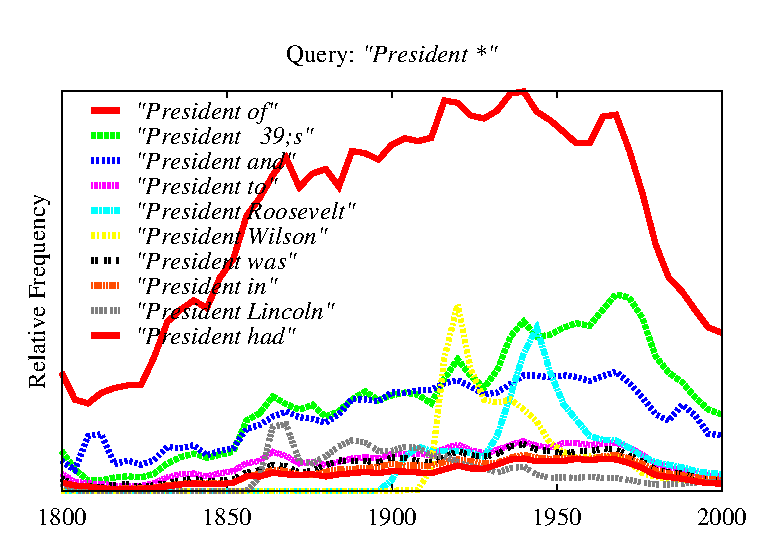
\includegraphics[width=0.49\textwidth]{graphs/president*_all}}
\hspace*{0.1cm}
\subfigure[1950-2000]{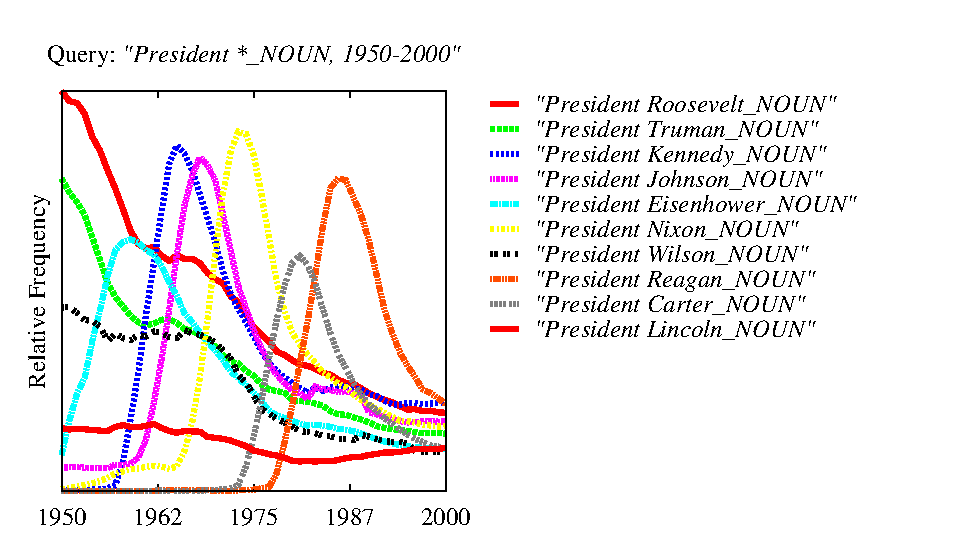
\includegraphics[width=0.49\textwidth]{graphs/President*1950}}

\hspace*{-0.5cm}\vspace*{-0.5cm}
\subfigure[1800-2000]{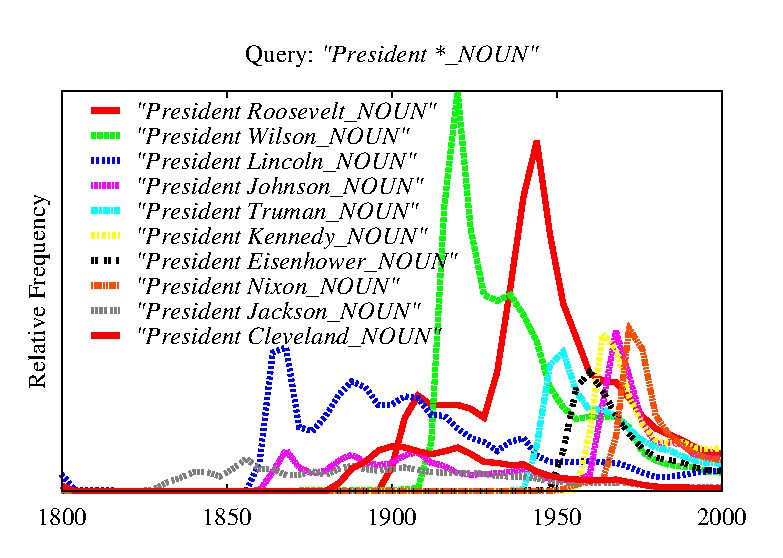
\includegraphics[width=0.69\textwidth]{graphs/President*1800}}
\hspace*{0.1cm}
\parbox[b][]{.28\textwidth}%
{\RawCaption{\caption{\label{fig:presidents}
Comparison of specification of POS tag in wildcard search}}}
\end{figure*}

% \begin{figure*}
% \label{fig:presidents}
% 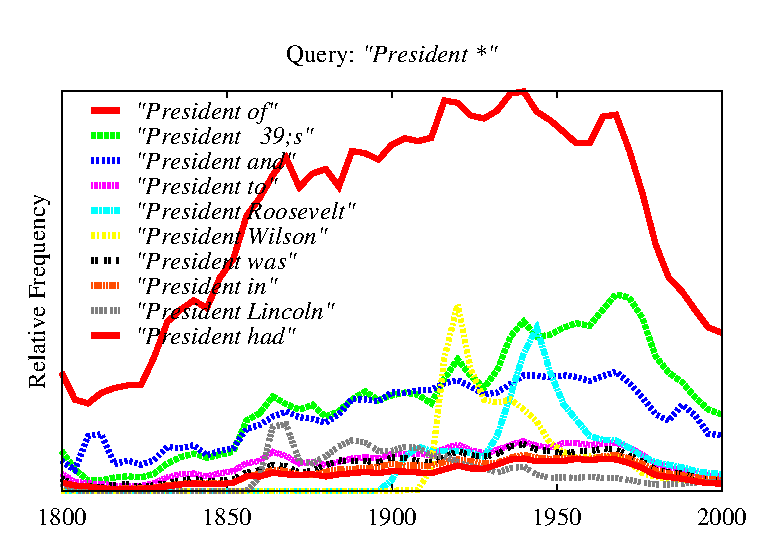
\includegraphics[width=.49\textwidth]{graphs/president*_all}
% 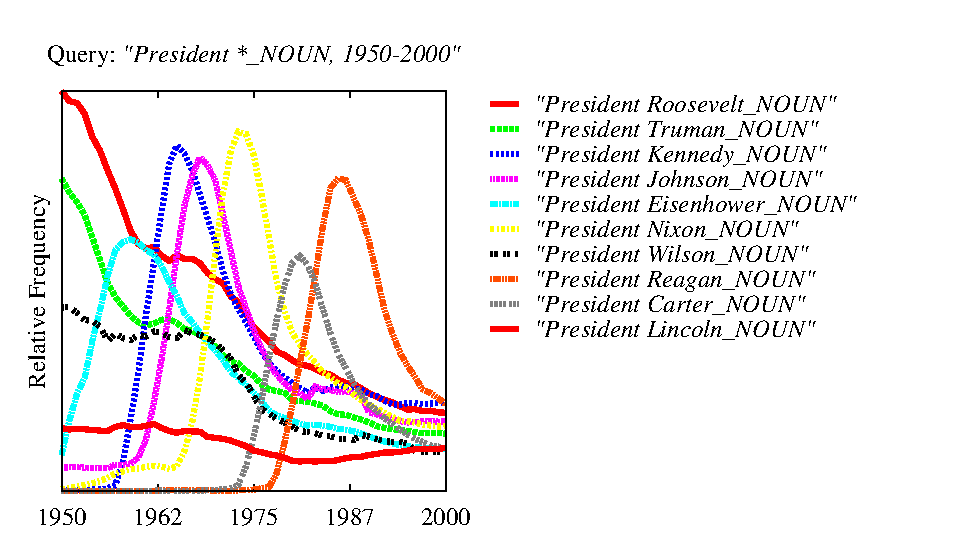
\includegraphics[width=.49\textwidth]{graphs/President*1950}\par
% 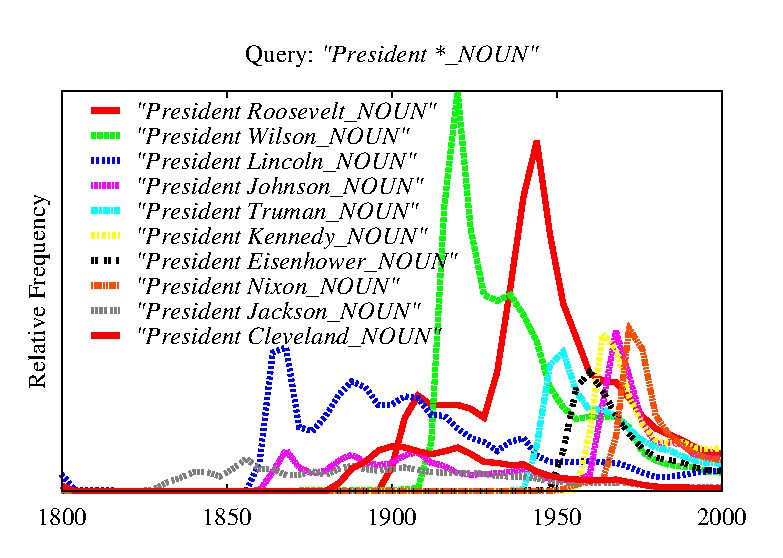
\includegraphics[width=.49\textwidth]{graphs/President*1800}
% \parbox[b][]{.49\textwidth}%
% % \RawCaption{
% \caption{Comparison of specification of POS tag in wildcard search}
% % }
% \end{figure*}


\section{Use Cases}
\label{sec:usecases}
\begin{figure}
\centering
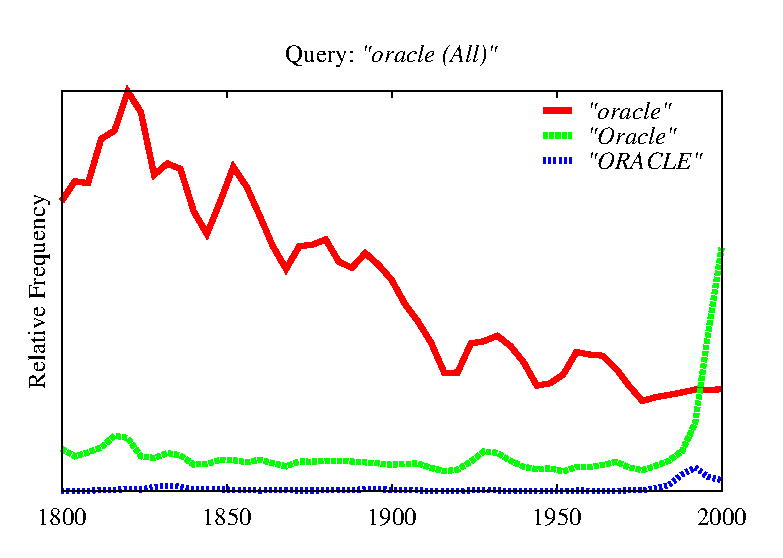
\includegraphics[width=.9\textwidth]{graphs/oracle}
\caption{\label{fig:apple} Discovery of Capitalization usage}
\end{figure}
The previous version of the Ngram Viewer brought the power of syntactic annotations and dependencies to the Ngram Corpus \cite{lin2012syntactic}, allowing for greater specificity when searching the corpus. The features we have added above continue this trend of specialization, but also provide the ability to group similar searches, preventing the need for overly verbose queries. Below we examine example uses of the new features independently and combined with those already present. We show specific queries here to highlight specific usages that we feel users will find the most beneficial, but wish to leave the analysis of the results to the experts.


\jmcomment{Not too happy with this next paragraph}
Before these features were added, queries the user could manually create queries to show the same charts, but that would require experimentation to find the most frequent ngrams out of the domain searched. Figure \ref{fig:manual president} shows a manually created query searching for specific presidents and upon comparison to Figure \ref{fig:presidents}, which is a wildcard query over the same time range, there is interesting data from presidents outside the time range that is left out.

The wildcard feature used on its own can be a powerful tool for the analysis of top expansions for a certain context.  Although it is powerful, we have found greater functionality from wildcards by their specification with POS tags. The user can attach an underscore and POS tag to either a wildcard-based or inflection based query to specify that the expansions returned should be a specific part of speech. Compare the utility of the generic wildcard and a search with a noun part-of-speech specification in a query examining president names, `\query{President *}'/`\query{President *\_NOUN}' shown in Figure \ref{fig:presidents}. The former gives a mixture of prepositions, particles, and verbs along with names of presidents, and because the latter specifies nouns the top expansions turn out to be names and more in line with the intention of the search. Also, note in Figure \ref{fig:presidents} the difference in expansions that searching over two different time ranges provides.



One of the primary benefits of capitalization searching is the combination of multiple searches in one. As in Figure \ref{fig:apple}, using capitalization searches allows for immediate identification of changing orthographic usage of a word or phrase, which in this case shows the arrival

\begin{figure*}
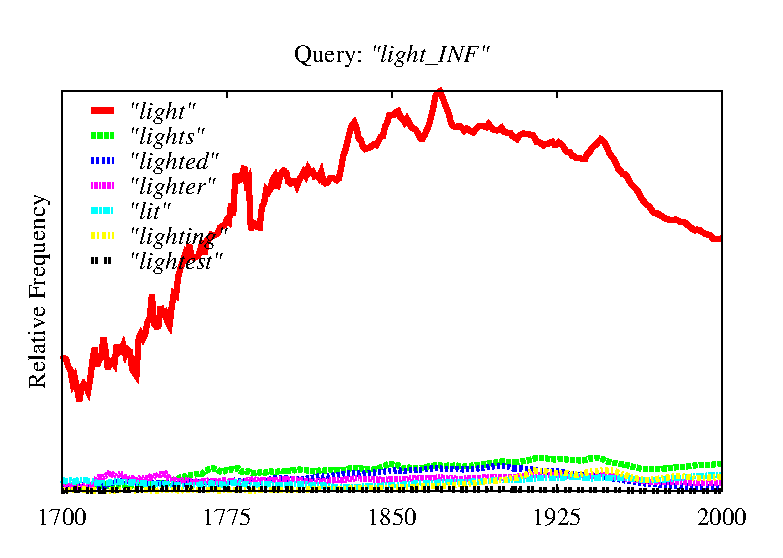
\includegraphics[width=.48\textwidth]{graphs/light_INF}
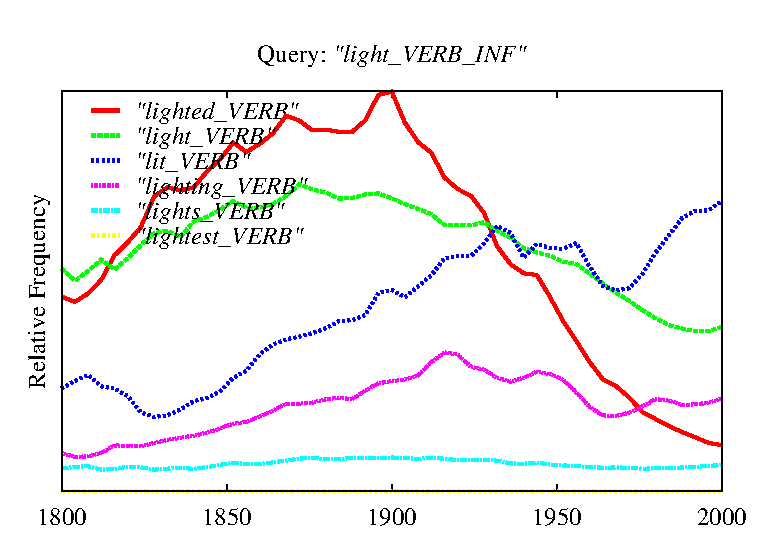
\includegraphics[width=.48\textwidth]{graphs/light_INF_VERB}
\caption{\label{fig:light} Comparison of specification of POS tag in wildcard search}
\end{figure*}
\eat{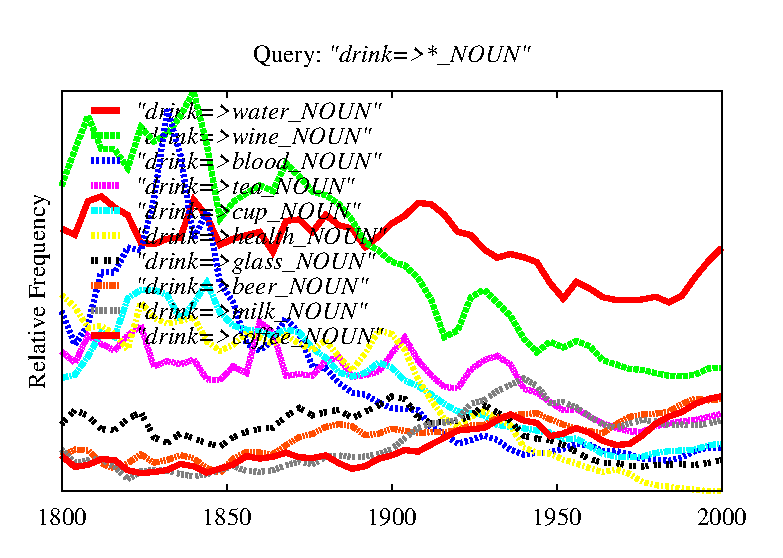
\includegraphics[width=.48\textwidth]{graphs/drink}
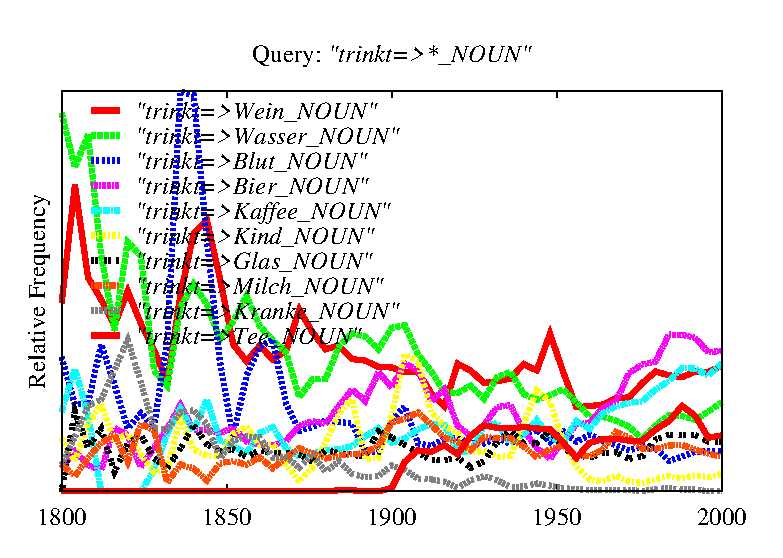
\includegraphics[width=.48\textwidth]{graphs/drink_GER}
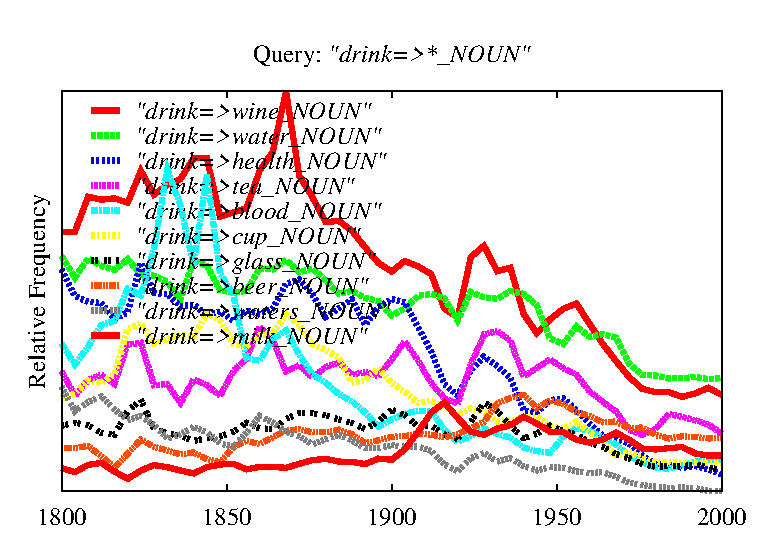
\includegraphics[width=.48\textwidth]{graphs/drink_UK}
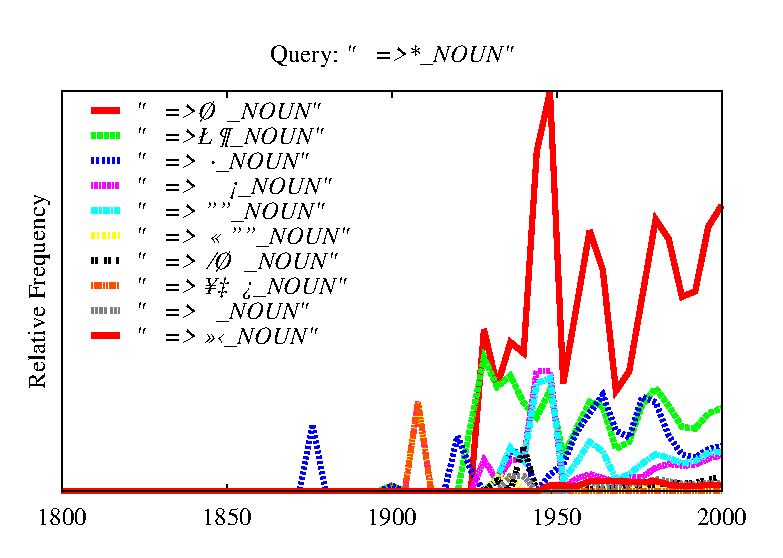
\includegraphics[width=.48\textwidth]{graphs/drink_CHI}
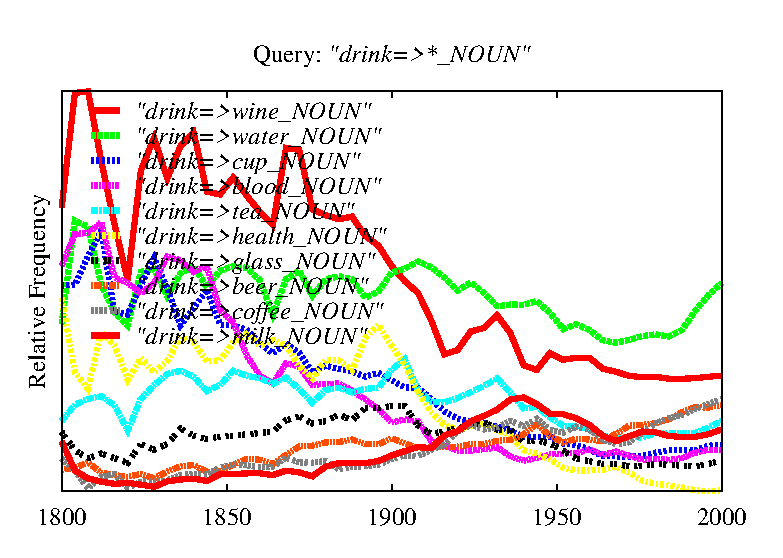
\includegraphics[width=.48\textwidth]{graphs/drink_USA}
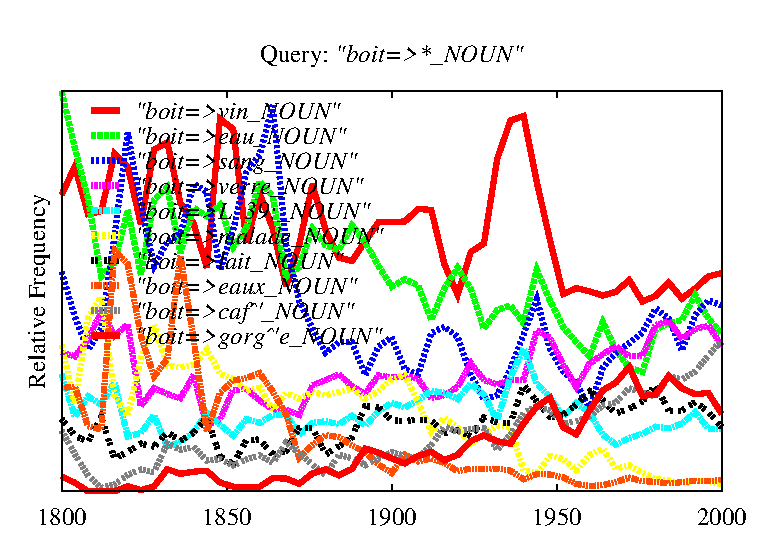
\includegraphics[width=.48\textwidth]{graphs/drink_FRE}
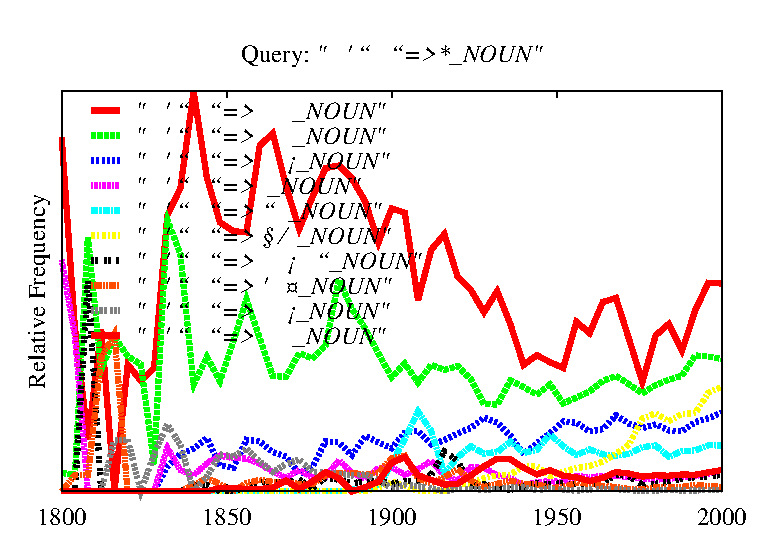
\includegraphics[width=.48\textwidth]{graphs/drink_HEB}
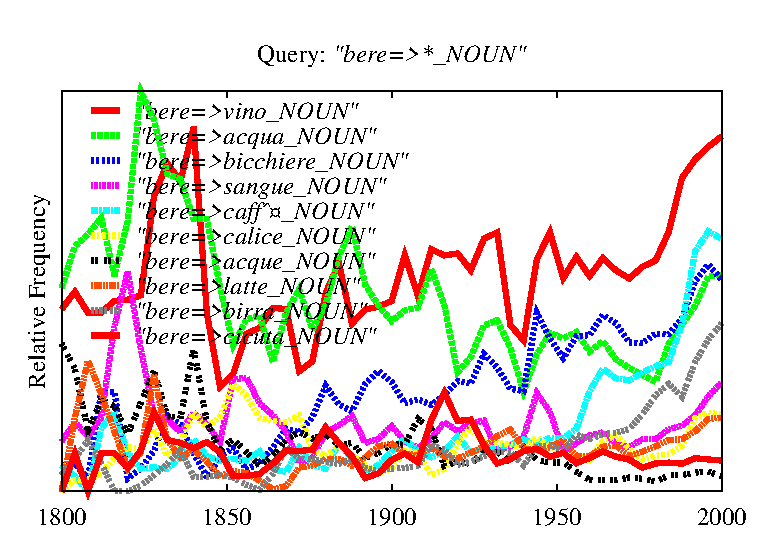
\includegraphics[width=.48\textwidth]{graphs/drink_ITA}
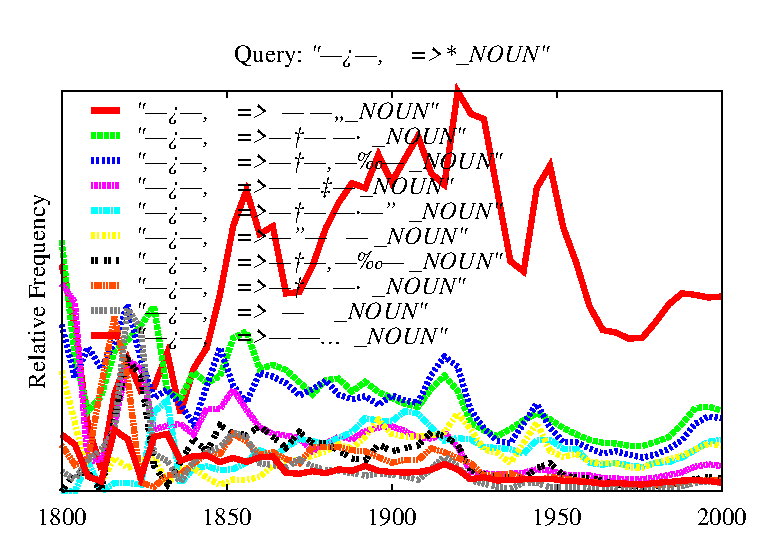
\includegraphics[width=.48\textwidth]{graphs/drink_RUS}
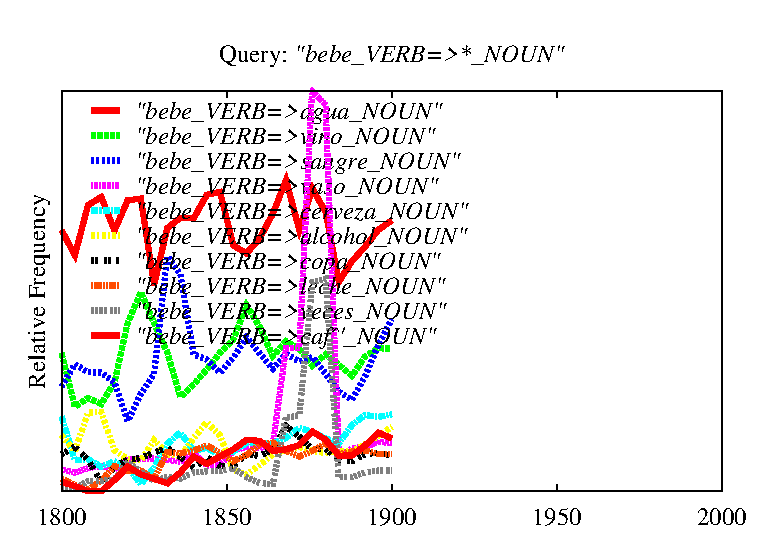
\includegraphics[width=.48\textwidth]{graphs/drink_SPA}}


\begin{table*}
\small
\centering
\begin{tabular}{|l|l|l|l|l|l|l|l|l|l|}
\hline
\begin{tabular}[c]{@{}c@{}} \textbf{English} \\ \textbf{(All)} \end{tabular}
&  \begin{tabular}[c]{@{}c@{}} \textbf{American} \\\textbf{English}\end{tabular} 
&  \begin{tabular}[c]{@{}c@{}} \textbf{British} \\\textbf{English}\end{tabular}
& \textbf{German}
& \textbf{French}
& \textbf{Russian}
& \hspace{1em}\textbf{Italian}
& \begin{tabular}[c]{@{}c@{}}\textbf{Chinese} \\ \textbf{(Simplified)}\end{tabular}
& \textbf{Spanish}
& \textbf{Hebrew} \\ \hline
\query{drink} & \query{drink} & \query{drink} & \query{trinkt} & \query{biore} & \textcyr{pit\char126} & \hspace{1em}\query{bere} & \begin{CJK}{UTF8}{gbsn}  \hspace{1.7em}喝 \end{CJK} & \query{beber} & \heb{לשתות}\\
\hline \hline
\begin{tabular}[c]{@{}c@{}}\query{water}\\ \query{wine}\\ \query{blood}\\ \query{tea}\\ \query{cup} 	\eat{\\ \query{health}\\ \query{glass}\\ \query{beer}\\ \query{milk}\\ \query{coffee}} \end{tabular} & 
\begin{tabular}[c]{@{}c@{}}\query{wine}\\ \query{water}\\ \query{cup}\\ \query{blood}\\ \query{tea} 	\eat{\\ \query{health}\\ \query{glass}\\ \query{beer}\\ \query{coffee}\\ \query{milk}}	\end{tabular} & 
\begin{tabular}[c]{@{}c@{}}\query{wine}\\ \query{water}\\ \query{health}\\ \query{tea}\\ \query{blood}	\eat{\\ \query{cup}\\ \query{glass}\\ \query{beer}\\ \query{waters}\\ \query{milk}}		\end{tabular} & 
\begin{tabular}[c]{@{}c@{}}\query{Wein} \\ \query{Wasser} \\ \query{Blut} \\ \query{Bier} \\ \query{Kaffee}	\eat{ \\ \query{Kind} \\ \query{Glas} \\ \query{Milch} \\ \query{Kranke} \\ \query{Tee}}	\end{tabular} &
\begin{tabular}[c]{@{}c@{}}\query{vin} \\ \query{verre} \\ \query{au} \\ \query{sang} \\ \query{lait}	\eat{ \\ \query{coup} \\ \query{caf}\'e \\ \query{h}\'e \\ \query{calice} \\ \query{aux}}	\end{tabular} & 
\begin{tabular}[c]{@{}c@{}} \textcyr{cha{\u i}} \\  \textcyr{vodu} \\  \textcyr{vino} \\  \textcyr{ego} \\  \textcyr{vodku}	
	\eat{ \\  \textcyr{kofe} \\  \textcyr{vina} \\  \textcyr{vody} \\ \textcyr{chashu} \\  \textcyr{emu}}	\end{tabular} & 
\begin{tabular}[c]{@{}c@{}}\query{vino} \\ \query{acqua} \\ \query{icchiere} \\ \query{sangue} \\ \query{caff}\'e	\eat{ \\ \query{calice} \\ \query{acque} \\ \query{latte} \\ \query{irra} \\ \query{cicuta}}	\end{tabular} & 
\begin{CJK}{UTF8}{gbsn} \begin{tabular}[c]{@{}c@{}}  \hspace{1em}酒 \\ \hspace{1em}  茶 \\ \hspace{1em}  水 \\ \hspace{1em}  咖啡 \\ \hspace{1em}  人	\eat{ \\ \hspace{1em}  别人 \\ \hspace{1em}  啤酒 \\ \hspace{1em}  女儿 \\ \hspace{1em}  烟 \\ \hspace{1em}  们 }	 \end{tabular} \end{CJK}& 
\begin{tabular}[c]{@{}c@{}}\query{agua} \\ \query{vino} \\ \query{\'a} \\ \query{sangre} \\ \query{aguas}	\eat{ \\ \query{vaso} \\ \query{cicuta} \\ \query{mas} \\ \query{leche} \\ \query{copa}}	\end{tabular} & 
\begin{tabular}[c]{@{}c@{}}  \hspace{.5em} \heb{יין}\\ \hspace{.5em} \heb{מים} \\ \hspace{.5em} \heb{כוס}\\ \hspace{.5em} \heb{ה} \\ \hspace{.5em} \heb{תה}	 \eat{\\ \hspace{.5em} \heb{קפה} \\ \hspace{.5em} \heb{כוסות} \\ \hspace{.5em} \heb{שכר} \\ \hspace{.5em} \heb{מיס}\\ \hspace{.5em} \heb{חלב}}	\end{tabular} \\ \hline
\end{tabular}
\caption{\label{tab:drink} Comparison of top dependencies from `drink' in all corpora\footnotemark{}}
\end{table*}
\footnotetext{Queries were initiated by translation from `drink' using Google Translate, and entered into the Ngram Viewer using the format \query{(drink)=>*\_NOUN}. Therefore the queries may not agree on tense/aspect/gender etc. across the different languages. }

\jmcomment{Automatic viewing of irregular vs regular verbs}




\section{Conclusions}
We have presented a new version of the Ngram Viewer with some new functionality. With the introduction of these new features, users can perform more powerful searches that show trends which were not possible to extract from earlier versions of the Viewer. The new features have been highlighted in a recent article by the Atlantic, as well on various blogs.

\jmcomment{Blog posts/entries from the internet:
http://sciencerefinery.com/2013/10/28/google-ngram-viewer-now-more-powerful-than-ever/
http://www.devingriffiths.com/google-books/google-n-gram-studies/
http://languagelog.ldc.upenn.edu/nll/?p=8472
http://www.textualscholarship.nl/?p=14051}

\section{Acknowledgements}
We would like to thank John DeNero, ...

\bibliographystyle{acl}
\bibliography{acl2014}
\end{document}
